\chapter{Game Theory Exercise 2}

\assignment{
  \textbf{Problem 2 - Multipath Routing} \\
  Imagine that there 4 nodes A, B, C and D linked as it is shown on the figure. User 1 would like to send his 
  data packets from B to D; user 2 would like to send his packets from A to C. First user can chose a route 
  B-A-D or B-C-D. There are also two choices for the second user: A-B-C and A-D-C. Throughput 
  experienced by a user depends on whether he is using a link alone or it is shared with another user. The 
  vectors (a; b) attached to each link denotes a throughput a user experiencing over the link: a if he is 
  doing it alone alone, and b if he shares it with another user.\\
  % Write a matrix to describe this game. Investigate if the game has Nash equilibrium and what would be a 
  % rational choice for the two users.  
  \begin{enumerate}
  \item Formulate in matrix representation.
  \item Find Nash equilibrium.
  \item What would be the rational choice?
  \end{enumerate}

  \begin{figure}[H]
    \centering
    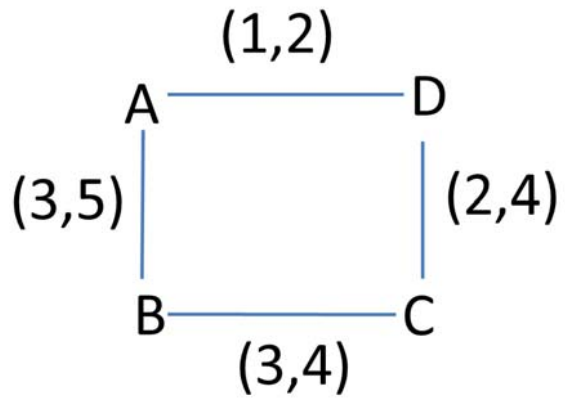
\includegraphics[width=0.35\textwidth]{gt_network_ex2.png}
  \end{figure}
}

\assignment{1. Formulate in matrix representation:} 
The matrix representation
  \begin{tabular}{ r|c|c| }
    \multicolumn{1}{r}{}
    &  \multicolumn{1}{c}{$s_2 = A-B-C$}
    & \multicolumn{1}{c}{$s_2 = A-D-C$} \\
    \cline{2-3}
    $s_1 = B-A-D$ & $(1,1)$ & $(1,2.5)$ \\
    \cline{2-3}
    $s_1 = B-C-D$ & $(2,1)$ & $(2,2)$ \\
    \cline{2-3}
  \end{tabular}

\assignment{2. Find Nash equilibrium:} 
The Nash equilibrium is $(2,2)$ where player 1 choose $B-C-D$ and player 2 choose $A-D-C$

\assignment{3. What would be the rational choice:}
The best for player 1 is $B-C-D$, and the best for player 2 is $A-D-C$
